\documentclass{beamer}

\mode<presentation>
\usetheme{Warsaw}
%\setbeamercolor{uppercol}{fg=white,bg=green!75!blue}

\definecolor{mygreen}{rgb}{.125,.5,.25}
\usecolortheme[named=mygreen]{structure}

\definecolor{lightgr}{rgb}{0.7 0.7 0.7}
\makeatletter
\addtobeamertemplate{footline}{%
  \color{lightgr}% to color the progressbar
  \hspace*{-\beamer@leftmargin}%
  \rule{\beamer@leftmargin}{2pt}%
  \rlap{\rule{\dimexpr
      \beamer@startpageofframe\dimexpr
      \beamer@rightmargin+\textwidth\relax/\beamer@endpageofdocument}{1.5pt}}
  % next 'empty' line is mandatory!

  \vspace{0\baselineskip}
  {}
}

\usepackage[OT2]{fontenc}
\usepackage{amsfonts,amssymb,amsthm,amsmath}
\usepackage{graphicx}
\usepackage{wrapfig}
\usepackage{subcaption}
\usepackage{multicol}

\def \zn{,\kern-0.09em,}
\setlength\intextsep{0pt}

\newcommand\eng{\fontencoding{OT1}\fontfamily{\rmdefault}\selectfont}
\newcommand\srb{\fontencoding{OT2}\fontfamily{\rmdefault}\selectfont}
\def\ug{\mathbin{\sphericalangle\,}}
\def\dj{d\kern-0.4em\char"16\kern-0.1em}
\def\Dj{\mbox{\raise0.3ex\hbox{-}\kern-0.4em D}}
\newcommand{\D}{\displaystyle}

\title{\textbf{Projekat iz rachunarstva}}
\author{Aleksa Vuchkovic1
\and
Lea Irt
\and 
Filip Jeremic1
}
\date{}
%\institute{Matematichka gimnazija, Beograd}

\begin{document}
\maketitle
\section{Zadatak}
\begin{frame}{Zadatak}
\begin{block}{}
Napisati program koji obradjuje podatke o rezultatima fudbalskih utamica korish${}$c1enjem jednostruko povezane liste. Podatke o rezultatima uchitati iz fajla u kom su podaci predstavljeni na sledec1i nachin, svaki rezultat u novoj liniji:      
Domac1in,Gost,broj golova domac1ina,broj golova gosta (na primer Crvena Zvezda,Partizan,1,1).\\
Napraviti meni za interakciju sa korisnikom preko konzole sa sledec1im opcijama koji se vrti sve dok korisnik ne izabere kraj rada:
\end{block}
\end{frame}
\begin{frame}{Zadatak}
\begin{itemize}
\item uchitavanje podataka iz fajla, ime fajla unosi korisnik, podaci se uchitavaju u neuredjenu listu
\item ispis svih utakmica iz liste 
\item ispis svih utakmica sa nereshenim rezultatom, ispisati utakmice i ukupan broj
\item brisanje utakmice gosta, korisnik unosi naziv tima i brishu se sve utakmice u kojima je on bio gost 
\item ispis poena za tim, korisnik unosi naziv tima, poeni se dodeljuju na sledec1i nachin 3-pobeda, 1-neresheno, 0-poraz
\item izlaz iz programa (obrisatu listu iz memorije)
\end{itemize}
\end{frame}

\begin{frame}{Ulazni fajl}
\begin{multicols}{2}
\scriptsize
\eng{
Man United,Leicester,2,1\\
Bournemouth,Cardiff,2,0\\
Fulham,Crystal Palace,0,2\\
Huddersfield,Chelsea,0,3\\
Newcastle,Tottenham,1,2\\
Watford,Brighton,2,0\\
Wolves,Everton,2,2\\
Arsenal,Man City,0,2\\
Liverpool,West Ham,4,0\\
Southampton,Burnley,0,0\\
Cardiff,Newcastle,0,0\\
Chelsea,Arsenal,3,2\\
Everton,Southampton,2,1\\
Leicester,Wolves,2,0\\
Tottenham,Fulham,3,1\\
West Ham,Bournemouth,1,2\\
Brighton,Man United,3,2\\
Burnley,Watford,1,3\\
Man City,Huddersfield,6,1\\
Crystal Palace,Liverpool,0,2\\
Arsenal,West Ham,3,1\\
Bournemouth,Everton,2,2\\
Huddersfield,Cardiff,0,0\\
Liverpool,Brighton,1,0\\
Southampton,Leicester,1,2\\
Wolves,Man City,1,1\\
Fulham,Burnley,4,2\\
Newcastle,Chelsea,1,2\\
Watford,Crystal Palace,2,1\\
Man United,Tottenham,0,3\\
Brighton,Fulham,2,2\\
Chelsea,Bournemouth,2,0\\
Crystal Palace,Southampton,0,2\\
Everton,Huddersfield,1,1\\
Leicester,Liverpool,1,2\\
Man City,Newcastle,2,1\\
West Ham,Wolves,0,1\\
Burnley,Man United,0,2\\
Cardiff,Arsenal,2,3\\
Partizan,Zvezda,10,0
}
\end{multicols}
\end{frame}

\section{}
\begin{frame}{Meni}
    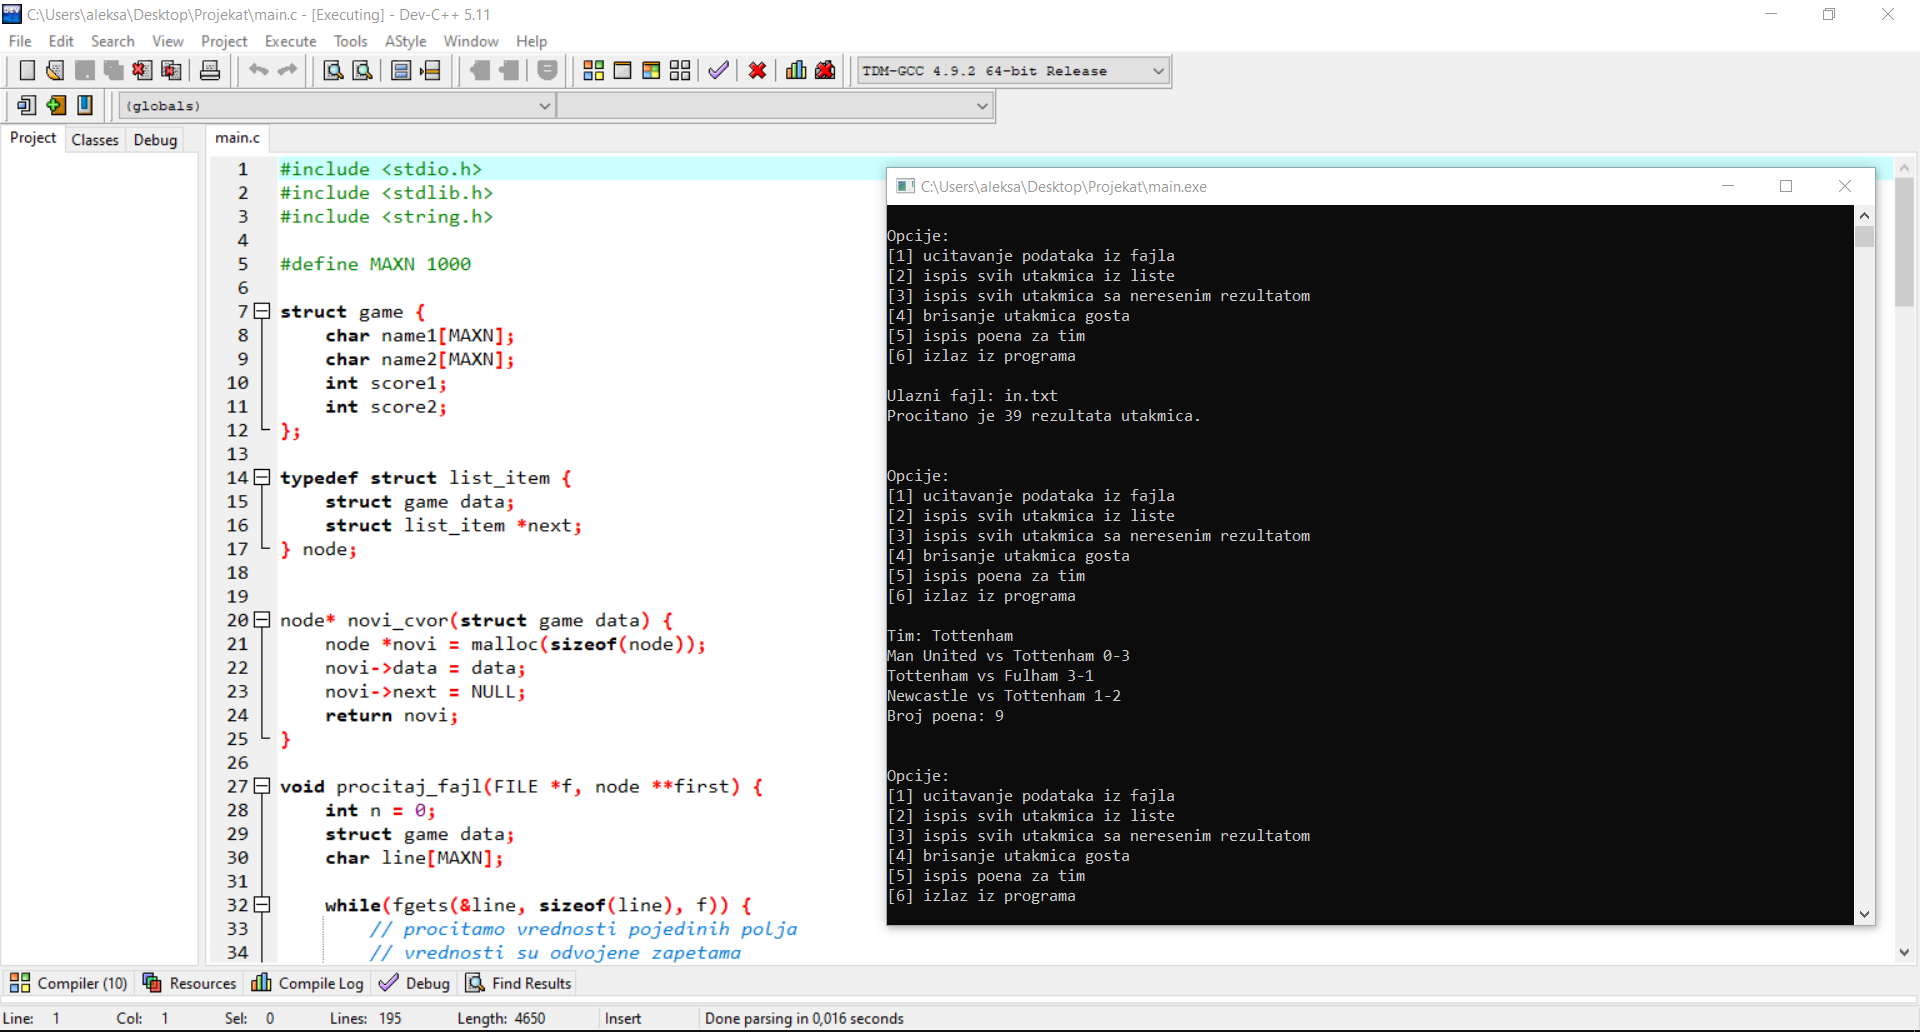
\includegraphics[scale=0.16]{projekat.png}
\end{frame}

\section{Reshenje}
\begin{frame}{Biblioteke i strukture}
\small\eng{
\begin{multicols}{2}
\#include $<$stdio.h$>$\\
\#include $<$stdlib.h$>$\\
\#include $<$string.h$>$\\

\#define MAXN 1000\\

struct game \{\\
    char name1[MAXN];\\
    char name2[MAXN];\\
    int score1;\\
    int score2;\\
\};\\

typedef struct list\_item \{\\
    struct game data;\\
    struct list\_item *next;\\
\} node;\\
\columnbreak
node* novi\_cvor(struct game data) \{\\
    node *novi = malloc(sizeof(node));\\
    novi-$>$data = data;\\
    novi-$>$next = NULL;\\
    return novi;\\
\}

\end{multicols}
}
\end{frame}

\begin{frame}{Chitanje fajla}
\scriptsize\eng{
\begin{multicols}{2}

void procitaj\_fajl(FILE *f, node **first) \{\\
    int n = 0;\\
    struct game data;\\
    char line[MAXN];\\
    while(fgets(line, sizeof(line), f)) \{\\
        // procitamo vrednosti pojedinih polja\\
        // vrednosti su odvojene zapetama\\
        char *p, *q;\\

        p = line;\\

        q = strchr(p, ',');\\
        *q = '$\backslash$0';\\
        strcpy(data.name1, p);\\
        p = q + 1;\\

        q = strchr(p, ',');\\
        *q = '$\backslash$0';\\
        strcpy(data.name2, p);\\
        p = q + 1;\\

        q = strchr(p, ',');\\
        *q = '$\backslash$0';\\
        data.score1 = atoi(p);\\
        p = q + 1;\\

        data.score2 = atoi(p);\\

        // napravimo cvor i dodamo na pocetak liste\\
        node *novi = novi\_cvor(data);\\
        novi-$>$next = *first;\\
        *first = novi;\\

        n++;\\
    \}\\

    printf("Procitano je \%d rezultata utakmica.$\backslash$n", n);\\
\}\\

\end{multicols}
}
\end{frame}

\begin{frame}{Ispis}
\eng{
\begin{multicols}{2}

void ispis(node *p) \{\\
    while(p != NULL) \{\\
        struct game item = p-$>$data;\\
        printf("\%s vs \%s \%d-\%d$\backslash$n", item.name1, item.name2, item.score1, item.score2);\\
        p = p-$>$next;\\
    \}\\
\}\\
\columnbreak
void ispis\_neresenih(node *p) \{\\
    while(p != NULL) \{\\
        struct game item = p-$>$data;\\
        if(item.score1 == item.score2)\\
            printf("\%s vs \%s \%d{}-\%d$\backslash$n", item.name1, item.name2, item.score1, item.score2);\\
        p = p-$>$next;\\
    \}\\
\}\\

\end{multicols}
}
\end{frame}

\begin{frame}{Broj poena za tim}
\scriptsize\eng{

int broj\_poena\_za\_tim(node *p, char *name) \{\\
    int z = 0;\\
    while(p != NULL) \{\\
        struct game item = p-$>$data;\\
        if(strcmp(item.name1, name)==0) \{\\
            printf("\%s vs \%s \%d{}-\%d$\backslash$n", item.name1, item.name2, item.score1, item.score2);\\
            if(item.score1 $>$ item.score2)\\
                z += 3;\\
            else if(item.score1 == item.score2)\\
                z += 1;\\
        \}\\
        else if(strcmp(item.name2, name)==0) \{\\
            printf("\%s vs \%s \%d{}-\%d$\backslash$n", item.name1, item.name2, item.score1, item.score2);\\
            if(item.score1 $<$ item.score2)\\
                z += 3;\\
            else if(item.score1 == item.score2)\\
                z += 1;\\
        \}\\
        p = p-$>$next;\\
   \}\\
    return z;\\
\}\\

}
\end{frame}

\begin{frame}{Brisanje liste ili njenog dela}
\scriptsize\eng{
\begin{multicols}{2}
int brisanje\_poena\_gosta(node **p, char *name) \{\\
    int z = 0;\\
    while(*p != NULL) \{\\
        struct game item = (*p)-$>$data;\\
        if(strcmp(item.name2, name)==0) \{\\
            node *t = *p;\\
            *p = (*p)-$>$next;\\
            free(t);\\
            z++;\\
        \}\\
        else\\
            p = \&(*p)-$>$next;\\
    \}\\
    return z;\\
\}\\
\columnbreak
void obrisi\_listu(node **p)\{\\
    while(*p != NULL) \{\\
        node *t = (*p)-$>$next;\\
        free(*p);\\
        *p = t;\\
    \}\\
\}\\

\end{multicols}
}
\end{frame}

\begin{frame}{\eng{Main}}
\scriptsize\eng{
int main()\\
\{\\
    int quit = 0;\\

    // lista\\
    node *first = NULL; // lista utakmica\\

    // fajl sa rezultatima\\
    FILE *f;\\
    char fn[MAXN];\\

    // ime tima\\
    char name[MAXN];\\

    while(!quit) \{\\
        printf("$\backslash$nOpcije:$\backslash$n");\\
        printf("[1] ucitavanje podataka iz fajla$\backslash$n");\\
        printf("[2] ispis svih utakmica iz liste$\backslash$n");\\
        printf("[3] ispis svih utakmica sa neresenim rezultatom$\backslash$n");\\
        printf("[4] brisanje utakmica gosta$\backslash$n");\\
        printf("[5] ispis poena za tim$\backslash$n");\\
        printf("[6] izlaz iz programa$\backslash$n$\backslash$n");\\

        char opcija = getch();\\
        

}
\end{frame}

\begin{frame}{\eng{Switch}\srb{ sa funkcijama}}
\scriptsize\eng{
\begin{multicols}{2}

        switch(opcija) \{\\
        case '1':\\
            // ako su rezultati vec procitani, prvo obrisi postojecu listu\\
            if(first != NULL)\\
                obrisi\_listu(\&first);\\

            printf("Ulazni fajl: ");\\
            gets(fn);\\

            f = fopen(fn, "r");\\
            procitaj\_fajl(f, \&first);\\
            fclose(f);\\
            break;\\
        case '2':\\
            ispis(first);\\
            break;\\
        case '3':\\
            ispis\_neresenih(first);\\
            break;\\
        case '4':\\
            printf("Tim: ");\\
            gets(name);\\
            printf("Brisano utakmica: \%d$\backslash$n", brisanje\_poena\_gosta(\&first,name));\\
            break;\\
        case '5':\\
            printf("Tim: ");\\
            gets(name);\\
            printf("Broj poena: \%d$\backslash$n", broj\_poena\_za\_tim(first,name));\\
            break;\\
        case '6':\\
            obrisi\_listu(\&first);\\
            quit = 1;\\
            break;\\
        \}\\
        printf("$\backslash$n");\\
    \}\\
    return 0;\\
\}
\end{multicols}
}
\end{frame}

\section{}
\begin{frame}
\centering\LARGE HVALA NA PAZHNJI!
\end{frame}
\end{document}